% % % FUNDAMENTAÇÃO TEÓRICA

% % Colocar os conhecimentos teóricos que fundamentam o trabalho para que o leitor possa apreciá-lo. Falar a respeito dos conceitos principais, mas levar em consideração que o relatório não é um livro-texto (não é necessário colocar 20 páginas explicando todos os sub-tópicos da área). Por outro lado, a falta de conceitos importantes também pode ser um problema. Usar como regra de decisão se deve colocar ou não algo a seguinte pergunta: este conceito é necessário para a compreensão do trabalho? Se sim, mantê-lo. Ainda, no que diz respeito a profundidade: colocar em profundidade os conceitos relacionados aos tópicos que seu trabalho vai utilizar mais diretamente na metodologia.

% %\section{Fundamentação Teórica}

% % O projeto deverá incluir especificações do instrumento como um todo e especificações dos blocos. A partir de uma aplicação e mensurando de interesse, do ponto de vista do instrumento como um todo, o grupo deverá definir a faixa de medições, a faixa de indicações, resolução do instrumento, precisão do instrumento, sensibilidade do instrumento, máxima frequência de interesse e qualquer outra especificação importante em nível de sistema.
% % O sensor deverá ser escolhido com base em 
% % dispositivos comercialmente disponíveis e que tenha saída analógica. 
% % Características relativas ao princípio de medição, 
% % a função de transferência (incluindo sensibilidade) 
% % e restrições relativas a frequência da saída deverão ser detalhadas.

% \subsection{K-meams}

% K-means é um algoritmo de agregação (\textit{clustering}), um subconjunto dos algoritmos não supervisionados. Seu objetivo é formar $k$ agregados (\textit{clusters}) para $n$ observações, onde cada observação pertence ao \textit{cluster} cujo centro é o mais próximo.

% \subsection{K-medoids}

% K-medoids é um algoritmo de agregação (\textit{clustering}) similar ao k-means. No entanto, diferentemente do método $k-means$, esse método utiliza como centro do cluster um dos dados de entrada (que é identificado como medoid).

% \subsection{Partitioning Around Medoids - PAM}

% O algoritmo PAM pode ser descrito brevemente como:
% \begin{enumerate}
%     \item Inicialização: selecionar aleatoriamente $k$ dos pontos de dados $m$ como os medoids
%     \item Atribuição: associar cada ponto de dados ao medoid mais próximo, com base na distância Minkowski (que é um caso geral da distância euclidiana)
%     \item Atualização: para cada medoid $j$ e para  cada ponto de dados $i$ associado a $j$, trocar $j$ e $i$ e computar o custo total da configuração (que é, a diferença média de $i$ para todos os pontos de dados associados a $j$). Selecione o medoid $j$ com o menor custo da configuração. Iterar entre os passos 2 e 3 até que não haja mudança nas atribuições.
% \end{enumerate}

% \subsection{Coeficiente Silhueta}

% É uma métrica para avaliação de clusters, como os produzidos pelo método k-means e PAM. A expressão $1 - (a/b)$ pode ser usada para determinar o Coeficiente de Silhueta é, que possui uma faixa é entre $-1$ e $1$, onde:
% \begin{itemize}
%     \item $a$: distância média de um dado específico em relação a todos os outros dados do mesmo cluster. Se o $a$ for pequeno, a coesão do cluster é boa, pois todos os dados estão muito próximos;
%     \item $b$: a distância média mais baixa de um dado específico em relação a todos os outros dados do cluster mais próximo.Se o $b$ for grande, a separação do cluster é boa, pois o cluster mais próximo está distante; os dados que formam o cluster mais próximo estão mais distantes. Assim, é mais difícil haver sobreposição de dados.
% \end{itemize}

% O $k$ que produz o maior coeficiente de Silhueta será considerado o ideal.

% \subsection{K-nearest neighbors (KNN)}

% K-nearest neighbors é um  algoritmo de classificação, um subconjunto dos algoritmos supervisionados.

% Depois que o modelo está treinado, podemos realizar a previsão de a que classe um novo dado pertence, considerando a(s) classe(s) de seu(s) vizinho(s) mais próximos.

% \subsection{K-fold}

% A validação cruzada é uma técnica que permite que os resultados do teste não sejam influenciados por uma decisão enviesada da separação dos dados de treino e validação. Os dados são separados, como no caso da Figura \ref{fig: Grid search cross validation}, em cinco lotes onde avaliamos a cada vez quatro lotes para treinamento e um para teste, e este um lote um é substituído a cada nova rodada. Então, tomamos como resultado do treinamento a média destas cinco rodadas de treinamento.

% %\textcolor{red}{Figura só largada aqui} como mostra a Figura como mostra a Figura \ref{fig: Grid search cross validation}.
% \begin{figure}[H]
%         \centering
%         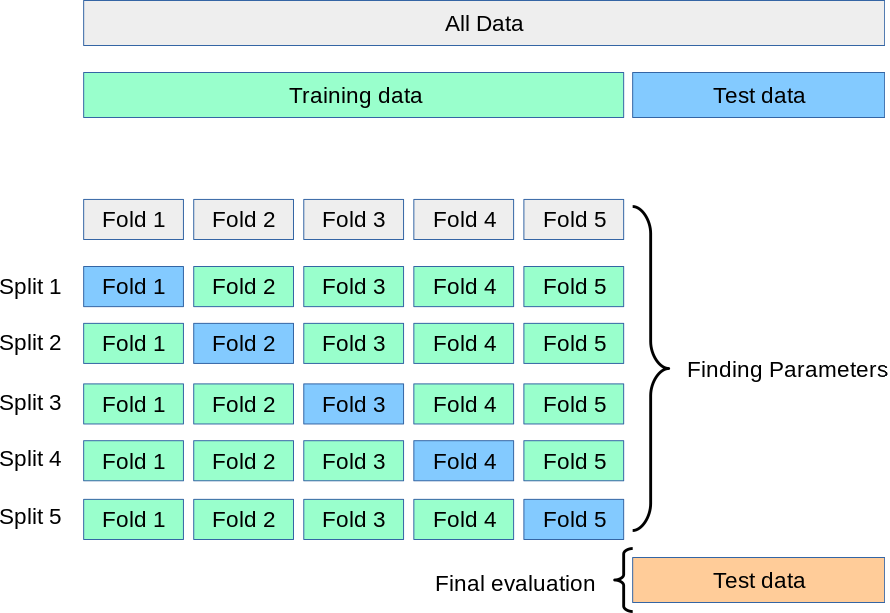
\includegraphics[width=0.75\textwidth]{Figuras/2. Fundamentação Teórica/grid_search_cross_validation.png}
%         \caption{Validação Cruzada (\textit{Grid search cross validation}).\\ \textbf{Fonte -} \cite{scikit-learn}}
%         \label{fig: Grid search cross validation}
% \end{figure}



% \subsection{Características do consumo de energia elétrica em uma residência}

% % Conforme \cite{zhang_forecasting_2018}, um número significativo de técnicas  tem sido utilizado para prever o consumo elétrico, incluindo redes neurais artificiais (ANN, do inglês \textit{Artificial Neural Networks}), máquinas de vetores de suporte (SVM, do inglês \textit{support-vector machine}), modelos auto-regressivo integrados de médias móveis (ARIMA, do inglês \textit{autoregressive integrated moving average}), modelos de regressão, técnicas de análise de agrupamento de dados (\textit{clustering techniques}) e \textit{empirical mode decomposition} (EMD). 
  
% Em seu estudo do impacto da granularidade do monitoramento temporal e espacial na \textit{performance accuracy} na previsão do consumo de energia de edifícios residenciais multi-familiares usando regressão vetorial de suporte (SVR, do inglês \textit{Support Vector Regression}), \cite{jain_forecasting_2014} encontrou como granularidade ótima intervalos temporais horários. Haviam sido testados intervalos  diários, horários e intervalos de $10$ minutos.

% \cite{zhang_forecasting_2018}, que também utilizou a técnica SVR,  destaca que, devido a natureza estocástica dos clientes residenciais individuais, a granularidade dos dados diários alcançou melhores resultados de previsão do que a granularidade horária em suas predições. A agregação do consumo horário ao diário é uma forma eficaz de mitigar o impacto da aleatoriedade nos comportamentos horários dos membros da família.

% % \cite{zhang_forecasting_2018}
% % 1) Data Cleansing
% % Some hourly data were missing and some were in wrong order in the meter readings. To avoid unexpected impacts on the prediction model, missing consumption cells were replaced by the average electrical consumption value of the previous and following hours, and the data were sorted chronologically. In the case of invalid/missing weather conditions or temperature/humidity data in the dataset downloaded from the government Web site, an average tem-perature/humidity value for the previous and following hours was calculated as a substitute for the missing hour. For an invalid weather condition (snow, cloudy, clear, etc.), the cell is filled using the last hour's weather condition.

% Sem a implementação de sensores comportamentais, alguns estudos, conforme \cite{zhang_forecasting_2018}, se concentraram na agregação de padrões de comportamento e abordagens de simulação estocástica para reconhecer e simular padrões comportamentais dos ocupantes com algoritmos de agregação.

% Quanto à seleção de características, \cite{zhang_forecasting_2018} aponta que \cite{beckel_revealing_cluster_2014} identificaram quatro categorias principais de fatores que afetam drasticamente o consumo de eletricidade: clima e localização, características de moradia, inventário de aparelhos e eletrônicos, e ocupação e comportamento. Adotando uma abordagem mais prática e viável, \cite{zhang_forecasting_2018} destaca que estudos recentes analisaram formas de usar variáveis temporais, tais como informações de calendário e variáveis e previsões meteorológicas, que podem ser obtidas de estações meteorológicas locais ou regionais.

% \cite{beckel_revealing_cluster_2014} utilizaram $5$ classificadores em seu estudo com diversas residências:
% \begin{itemize}
%     \item kNN, com $k = 5$ e como métrica de distância a distância euclidiana, do \textit{Add-On} \textit{Statistics toolbox} do \MATLAB;
%     \item \textit{Linear Discriminant Analysis} (LDA), do \textit{Add-On} \textit{Statistics toolbox} do \MATLAB;
%     \item \textit{Mahalanobis
% distance classifier}, do \textit{Add-On} \textit{Statistics toolbox} do \MATLAB;
%     \item classificador SVM (implementação LIBSVM);
%     \item AdaBoost, do \textit{Add-On} \textit{Statistics toolbox} do \MATLAB;
% \end{itemize}


% % B. Performance Measures
% \subsubsection{Métrica MAPE em estudos de predição de consumo elétrico}

% Para determinar a performance da predição de seu modelo, \cite{zhang_forecasting_2018} utilizaram o \textit{Mean Absolute Percentage of Error} (MAPE) para validação. Os autores destacam que a métrica MAPE é amplamente utilizada para medir a \textit{accuracy} da previsão em estudos de predição de eletricidade.

% \begin{equation}
%     \text{MAPE (\%)} = \dfrac{100}{n} \sum_{j=1}^{n} \left| \dfrac{y_j - \hat{y_j}}{y_j} \right|
% \end{equation}, 
% onde:
% \begin{itemize}
%     \item $y_i$ é o consumo de eletricidade real da casa $j$;
%     \item $y_i$ é o consumo de eletricidade predito;
%     \item $n$ é o número de observações.
% \end{itemize}
